\chapter{Struktura sustava}
\label{pog:struktura_sustava}

Svrha cjelokupnog sustava je okidanje obavljanja određenog procesa, tj. signalizacija
za početak obavljanja nekog posla glasom. Također, sustav mora biti sposoban pokrenuti
proces u bilo kojem trenutku, a odaziv bi trebao biti trenutačan što
znači da cijeli proces prikupljanja zvuka, obrade te izvršavanja mora raditi
kontinuirano u stvarnom vremenu. Srce sustava, tj. dio koji je zadužen za
samo prepoznavanje određene naredbe je neuronska
mreža trenirana na skupu zvučnih zapisa koji sadrže željene naredbe, a čija je struktura
detaljnije objašnjena u poglavlju o neuronskoj mreži \ref{pog:neuronska_mreza}.
Shodno tome, sustav je izgrađen od četiri modularna
podsustava implementirana na mikrokontroleru:

\begin{itemize}
    \item Akvizicija zvuka
    \item Generiranje značajki
    \item Aktivacija neuronske mreže
    \item Prepoznavanje i aktivacija naredbi
\end{itemize}

Ideja u pozadini navede podjele je lakša prilagodba cjelokupnog
sustava na različite mikrokontrolerske platforme, drugačiju obradu
akviziranog zvuka, korištenje drugačije neuronske mreže ili samo 
kreiranje specifičnog zadatka koji će se aktivirati određenom naredbom.
Na slici \ref{pic:struktura_sustava} grafički je prikazan opisani sustav.

\begin{figure}[htb]
    \centering
    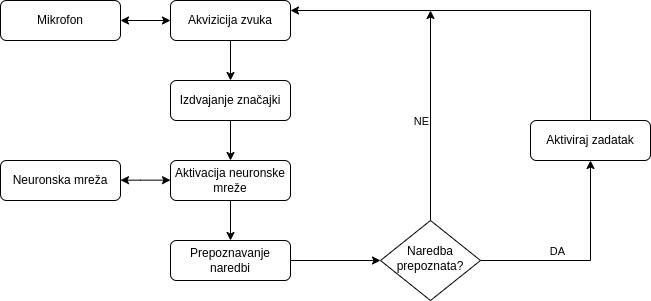
\includegraphics[width=1\linewidth]{Chapters/struktura_sustava/struktura_sustava.png} 
    \caption{Struktura sustava na mikrokontroleru\cite{flowchart}}
    \label{pic:struktura_sustava}
\end{figure}

\section{Akvizicija zvuka}
\label{sec:acq}

Podsustav za akviziciju zvuka je usko vezan uz platformu na kojoj
je sustav implementiran zbog toga što je zadužen za komunikaciju 
sa sustavom koji prikuplja stvarne signale sa senzora (mikrofona).
ESP32 Lyrat Development Board \cite{lyrat}, na kojem je sustav
implementiran, na sebi ima već ugrađen mikrofon i audio kodek
s kojim je moguće komunicirati putem I2S protokola. Na slici
\ref{pic:esp} prikazan je blok dijagram ESP32 razvojne platforme.

\begin{figure}[htb]
    \centering
    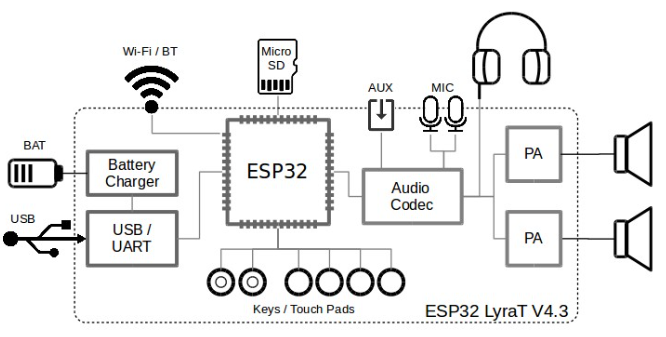
\includegraphics[width=0.75\linewidth]{Chapters/struktura_sustava/akvizicija/lyrat.png} 
    \caption{ESP32 Lyrat \cite{lyrat}}
    \label{pic:esp}
\end{figure}

Najvažniji dio razvojne platforme je upravo ESP32-WROVER-E mikrokontroler
na kojem je cjelokupni sustav za prepoznavanje govornih naredbi 
implementiran. Upravo on je zadužen za komunikaciju s ES8388 
audio kodekom \cite{es8388}. ES8388 je integrirani sklop koji na spomenutoj
platformi služi za analogno-digitalnu (engl. \textit{ADC}) te digitalno-analognu 
(engl. \textit{DAC}) pretvorbu, tj. upravljanje audio ulazom (mikrofon) te audio
izlazom (AUX priključak). Mikrokontroler putem I2C sučelja konfigurira kodek,
dok konkretne zvučne signale uzima putem I2S sučelja. Budući da je ESP32 Lyrat
platforma prilagođena razvoju audio sustava, konfiguracija i puštanje u pogon
akvizicije zvuka je vrlo jednostavno. U programskom kodu \ref{code:ES8388init}
prikazana je inicijalizacija kodeka.\\

\begin{lstlisting}[language=C++, caption=Inicijalizacija kodeka, label=code:ES8388init]
    audio_board_handle_t board_handle = audio_board_init();
    audio_hal_ctrl_codec(board_handle->audio_hal, AUDIO_HAL_CODEC_MODE_ENCODE, AUDIO_HAL_CTRL_START);
\end{lstlisting}

Sav posao koji se nalazi iza prikazanih naredbi, obavlja ESP-ADF
(engl. \textit{Espressif Audio Development Framework}). To je biblioteka koja pojednostavljuje
razvoj aplikacija vezanih za obradu zvuka kao što je akvizicija, kodiranje i 
dekodiranje različitih formata audio zapisa te komunikacija s računalom ili 
memorijskom karticom.
Nakon inicijalizacije kodeka i definiranja konfiguracije postavki I2S komunikacije,
potrebno je samo pokrenuti protočni akvizicijski sustav (engl. \textit{pipeline}), 
a to je prikazano u programskom kodu \ref{code:pipeline}.\\

\begin{lstlisting}[language=C++, caption=Pokretanje akvizicijskog sustava, label=code:pipeline]
    ESP_LOGI(TAG, "Creating i2s stream");
    audio_element_handle_t i2s_stream_reader;
    i2s_stream_cfg_t i2s_cfg = I2S_STREAM_CFG_DEFAULT();
    i2s_cfg.type = AUDIO_STREAM_READER;
    i2s_cfg.i2s_port = I2S_NUM_0;
    i2s_cfg.i2s_config = i2s;
    i2s_stream_reader = i2s_stream_init(&i2s_cfg);

    ESP_LOGI(TAG, "Creating audio pipeline");
    audio_pipeline_handle_t pipeline;
    audio_pipeline_cfg_t pipeline_cfg = DEFAULT_AUDIO_PIPELINE_CONFIG();
    pipeline = audio_pipeline_init(&pipeline_cfg);
    audio_pipeline_register(pipeline, i2s_stream_reader, "i2s");
    audio_pipeline_run(pipeline);
\end{lstlisting}

Frekvencija otipkavanja postavljena u konfiguraciji iznosi 16000 Hz što
je dovoljno za ovakav tip sustava \cite{wardentinyml}.
Nakon pokretanja akvizicijskog podsustava, sve što je preostalo je uzimati nove
podatke s kraja protočne strukture podsustava. Konstantno uzimanje novih podataka, tj. komunikacija
s ES8388 kodekom, odvojeno je u posebnu dretvu. Na taj način programski je 
odvojena akvizicija sirovih podataka (sirovi u smislu da nisu još obrađeni ni
na kakav način) od ostatka sustava. Ovaj podsustav je proizvođač novih podataka,
dok je ostatak sustava potrošač (također jednodretven). Sve što je preostalo je
ubaciti pouzdan i efikasan način komunikacije između njih. Za tu svrhu odabran je
kružni međuspremnik (engl. \textit{ring buffer}). On omogućuje asinkrono pisanje u njega
te čitanje iz njega. Implementacija takve strukture dostupna je unutar FreeRTOS-a 
\cite{ringbufferrr}. 


\begin{lstlisting}[language=C++, caption=Razred AudioRecorder, label=code:AudioRecorder]
class AudioRecorder
{
    private:
        uint32_t sampleRate;
        RingbufHandle_t ringBuffer;
        TaskHandle_t captureAudioHandle;
        static void captureAudioTask(void* pvParameters);
    public:
        AudioRecorder(uint32_t sampleRate) : sampleRate(sampleRate), 
                                             ringBuffer(NULL), 
                                             captureAudioHandle(NULL) {}
        uint32_t getSamples(int16_t* samples, size_t numOfSamples);
};
\end{lstlisting}

Opisani podsustav za akviziciju u programskom kodu zapakiran je u razred imena 
AudioRecorder \ref{code:AudioRecorder}. Prema van, razred nudi metodu potpisa
\texttt{uint32\_t getSamples(int16\_t* samples, size\_t numOfSamples)} koja 
omogućuje dohvaćanje proizvoljnog broja \texttt{uint16\_t} podataka jer 
se akvizirani zvučni signal sprema upravo u tom obliku. Zbog ovakve strukture
ovog podsustava, sve što je potrebno u glavnoj petlji sustava je stvaranje objekta
razreda AudioRecorder, alociranje spremnika za dohvaćanje podataka te kontinuirano
pozivanje opisane funkcije koja kao argumente prima pokazivač na alocirani spremnik
te željeni broj audio uzoraka.

Spomenuta modularnost ostvarena je tako što je cijela funkcionalnost akviziranja
novih zvučnih uzoraka sadržana u opisanom razredu. Pokretanje cjelokupnog sustava
na drugoj platformi koja ima drugi audio kodek, drugačiji mikrofon ili se samo 
radi o drugom mikrokontroleru bit će moguće pisanjem novog razreda koji
prati zadano sučelje.
\section{Generiranje značajki}
\label{sec:gen}

Generiranje značajki je drugi podsustav spomenut u uvodnom dijelu, također
prikazan na slici \ref{pic:struktura_sustava}. Nakon što je omogućena akvizicija
zvučnih uzoraka, potrebno ih je obraditi kako bi se mogli predati neuronskoj mreži 
na klasifikaciju. Naime, modeli strojnog učenja (kao što je neuronska mreža) rade
s različitim primjerima podataka. Razlikovanje primjera temelji se na odredivanju
različitih značajki ulaznih podataka. Klasičan primjer koji se koristi kako bi se 
približio pojam značajki jest model predikcije cijene nekakve
nekretnine. U tom slučaju značajke koje bi model mogao koristiti su lokacija,
godina izgradnje, površina, razina energetske učinkovitosti i slično. Medutim, što
bi bile značajke našeg ulaznog toka signala? Možemo, ispostavit će se naivno, uzeti
amplitudu svake vrijednosti. U slučaju da promatramo period od jedne sekunde
signala s već spomenutim otipkavanjem od 16 kHz, broj značajki koje bi naš model
morao ”progutati” jest 16000. Obraditi toliku količinu podataka u jako kratkom
vremenu (sustav mora raditi bez konstantno i bez mrtvog vremena) na resursno
ograničenom sustavu kao što je mikrokontroler ne zvuči obećavajuće. Nekako sve 
upućuje na to da je potrebno na neki način prilagoditi ulazni signal, tj. izvući
iz signala bitne informacije i tako smanjiti veličinu podataka. 

\subsection{Model govora}
\label{sec:speech}

Kako bismo identificirali kojim značajkama bi bilo korisno opisati ljudski govor,
potrebno je na neki način modelirati nastanak glasa. Prilikom govorne komunikacije,
pluća govornika se pod djelovanjem mišića prsnog koša stišću i potiskuju zrak kroz
vokalni trakt čiji su glavni dijelovi prikazani na slici \ref{pic:glas}.

\begin{figure}[htb]
    \centering
    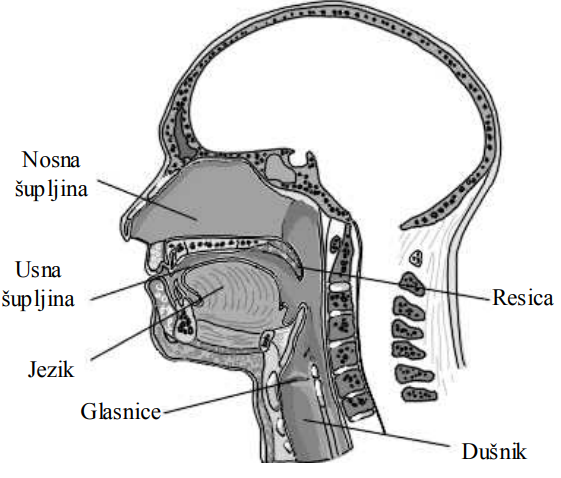
\includegraphics[width=0.6\linewidth]{Chapters/struktura_sustava/generiranje_znacajki/glas.png} 
    \caption{Presjek glave i osnovni dijelovi vokalnog trakta koji sudjeluju u produkciji govornog signala \cite{petrinovic2002}}
    \label{pic:glas}
\end{figure}

Glasnice (engl. glottis) su vrlo značajan organ u procesu formiranja govora. 
Ponašaju se kao mehanički
oscilator koji prelazi u stanje relaksacijskih oscilacija uslijed struje zraka iz pluća koja kroz njih
prolazi. Na frekvenciju njihovog titranja utječu brojni parametri, a među najznačajnijim su
pritisak zraka iz pluća na ulazu u glasnice i napetost samih glasnica.
Takvim periodičkim titranjem, glasnice formiraju periodičku struju zraka, tj. 
kvazi-periodične impulse (engl. glottal pulse) koja zatim prolaze kroz ostatak 
vokalnog trakta što vodi do stvaranja artikuliranih glasova. U slučaju da 
su glasnice potpuno opuštene, neće
doći do oscilacija i struja zraka iz pluća će neometano prolaziti kroz vokalni trakt 
(tada se ne formira kvazi-periodični impuls, nego je rezultat prolaska zraka kroz glasnice
slučajni šum, a rezultat cijelog procesa je stvaranje neartikuliranih glasova). 

S druge strane, vokalni trakt se ponaša kao filtar koji spektralno mijenja karakteristiku
pobudnog signala (engl. vocal tract frequency response). 
Geometrijom vokalnog trakta, koja se mijenja ovisno o položaju 
artikulatora kao što su jezik, usne, čeljust i resica, bit će određen ton (visina i
spektralni sastav) formiranog signala (govora) \cite{petrinovic2002}. 

Jednostavni model koji se koristi u području obrade prirodnog govora je da se on 
može prikazati kao izlaz iz linearnog, vremenski promjenjivog sustava čija se 
svojstva sporo mijenjaju s vremenom. Međutim, ako se promatraju dovoljno kratki
segmenti govornog signala, svaki se segment može učinkovito modelirati kao izlaz
iz linearnog, vremenski invarijantnog sustava pobuđenog bilo
kvazi-periodičnim impulsima bilo slučajnim šumom (engl. random noise signal).
Opisani sustav može se prikazati jednadžbom \ref{eq:govor}

\begin{equation}
    X(f) = E(f) \cdot H(f)
    \label{eq:govor}
\end{equation}

gdje je:
\begin{itemize}
    \item \(X(f)\) odziv sustava (govor),
    \item \(E(f)\) pobuda (kvazi-periodični impuls),
    \item \(H(f)\) prijenosna funkcija vokalnog trakta.
\end{itemize}

U vremenskoj domeni isti sustav može se prikazati jednadžbom \ref{eq:govor_vremenska}.
Množenju u frekvencijskoj domeni istovjetna je konvolucija u vremenskoj (i obratno!).

\begin{equation}
    x(t) = e(t) \ast h(t)
    \label{eq:govor_vremenska}
\end{equation}

Cilj ovakvog modeliranja je pronaći bitne informacije u govornom signalu. Pretpostavka na
kojoj se temelji daljnji rad je da je skoro sva informacija iz govornog signala sadržana
u prijenosnoj funkciji govornog trakta, tj. pobuda (kvazi-periodični impulsi) ostaje
konstantnna tijekom govora (veliko pojednostavljenje, međutim svi modeli na kojima
se temelji ovo područje zasnivaju na ovoj činjenici \cite{multiplier, emotion, sidhu2024mfcc}).
Zbog toga želimo pronaći način za 
razdvajanje tih dvaju elemenata modela. Ako primijenimo logaritamsku funkciju na
sustav opisan u frekvencijskoj domeni proizlazi \ref{eq:logaritam}.

\begin{equation}
    \label{eq:logaritam}
    \begin{aligned}
        \log(X(f)) &= \log(E(f) \cdot H(f)) \\
        \log(X(f)) &= \log(E(f)) + \log(H(f))
    \end{aligned}
\end{equation}

Prikazanim su uspješno razdvojeni elementi modela, tj. vidljiv je rastav na zbrojnike
ako se primijeni logaritamska skala. Na slici \ref{pic:rastav} prikazan je utjecaj
komponenata modela na konačni rezultat, a to je glas (engl. speech). 

\begin{figure}[htb]
    \centering
    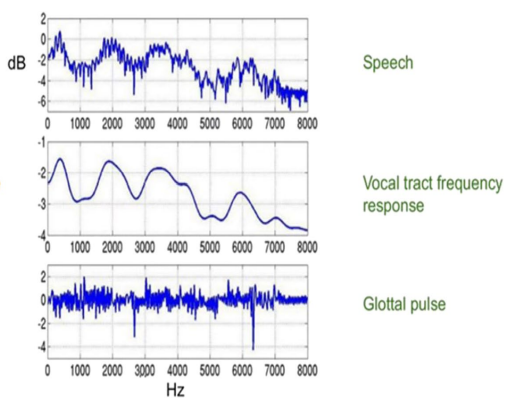
\includegraphics[width=0.6\linewidth]{Chapters/struktura_sustava/generiranje_znacajki/log.png} 
    \caption{Glasovni signal rastavljen na pobudu i odziv vokalnog trakta \cite{sidhu2024mfcc}}
    \label{pic:rastav}
\end{figure}

Jedino što preostaje je pronaći način za što efikasniji opis odziva vokalnog trakta. On će
u konačnici predstavljati zvučne zapise na kojima će model neuronske mreže biti treniran.
U području automatskog prepoznavanja govora te identifikaciji govornika uvelike se koriste
Mel kepstralni koeficijenti.


\subsection{MFCC}
\label{MFCCconstruction}
Mel kepstralni koeficijenti (engl. Mel frequency cepstral coefficients ili MFCC), tj. mjera 
euklidske udaljenosti MFCC vektora jedna je od najčešće korištenih mjera u automatskom 
prepoznavanju govora i govornika \cite{vasilijevic2011perceptual}. 
MFC koeficijenti (koji čine MFC vektor) pokazali su se odličnim načinom za spremanje informacije
koja je sadržana u govoru, a konkretno predstavljaju kratkotrajni spektar snage glasovnog 
signala. Naš sustav za prepoznavanje govornih naredbi će koristiti upravo njih za 
značajke koje predstavljati zvučni signal akviziran pomoću podsustava za akviziciju. 
Najbolji način za opis ovih koeficijenata je prikaz postupka kojim se dobivaju.


\subsubsection{Preklapajući prozori}
\label{sec:win}
Izlaz iz podsustava za akviziciju je signal koji predstavlja zvuk iz okoline uređaja, 
a nove uzorke je moguće dobiti kontinuiranim pozivima prikladne metode tog podsustava
na način opisan u poglavlju \ref{sec:acq}. Kontinuirani dotok novih uzoraka potrebno 
je uokviriti, tj. uzimati određeni broj uzoraka, obraditi ih te opet uzeti novije uzorke. 
Pozadina ovakvog pristupa opisana je u poglavlju \ref{sec:speech} u kojem je predstavljen
model nastajanja govora. Naime, kako bi takav model dobro radio, potrebno je promatrati
kratke isječke signala u kojima su ton i visina signala stabilni. Također, potrebno je
ne uzeti svaki put cijeli okvir novih uzoraka, nego, u svrhu boljeg očuvanja informacije,
ostaviti određeni broj uzoraka iz starog okvira. Na taj način, dobili smo prozor (engl. window)
koji se pomiče po akviziranom signalu, tj. svaki sljedeći je jednim dijelom preklopljen
preko prošlog što je prikazano na slici \ref{pic:sliding}. Zelenom bojom je obojan prozor
u iteraciji nakon prozora obojanog svijetlosmeđom bojom. Određeni dio uzoraka je isti,
a određeni dio su novi uzorci dobiveni od podsustava za akviziciju.

\begin{figure}[htb]
    \centering
    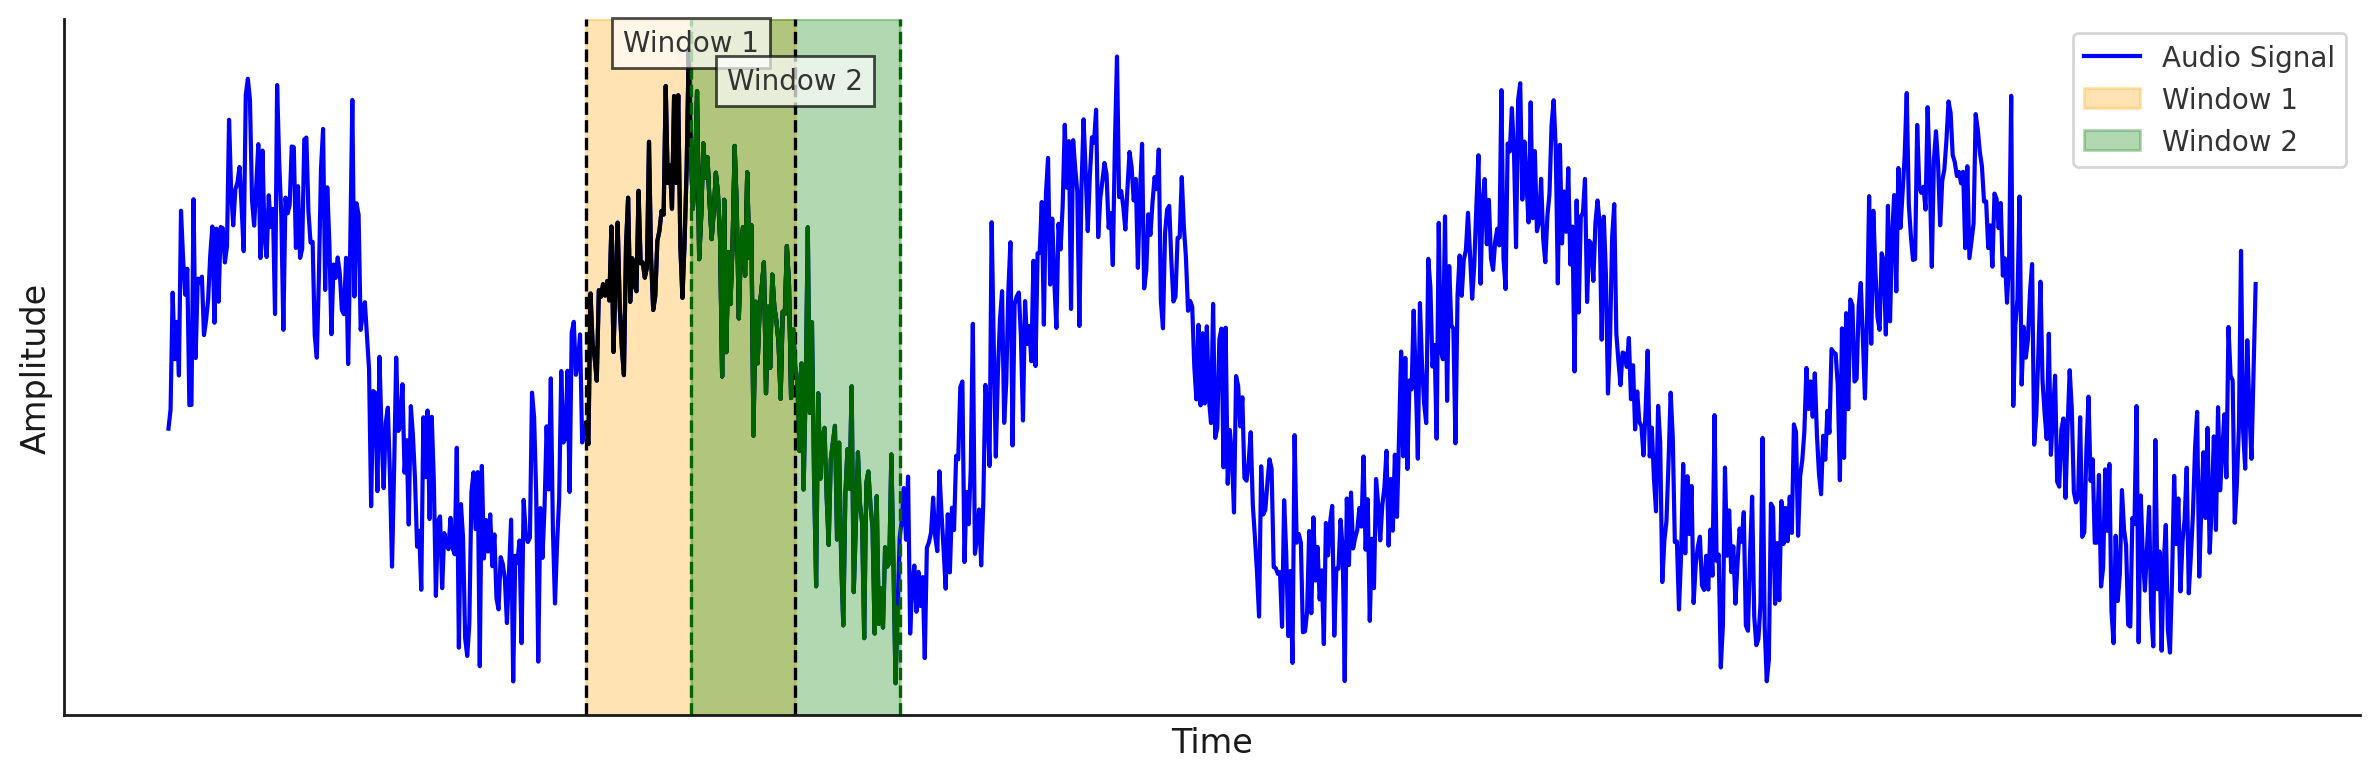
\includegraphics[width=0.8\linewidth]{Chapters/struktura_sustava/generiranje_znacajki/sliding.png} 
    \caption{Preklapajući prozori}
    \label{pic:sliding}
\end{figure}

U glavnoj petlji programskog koda inicijalizirano je polja koje sprema nove uzorke te 
polje koje zaduženo za spremanje trenutnog prozora podataka. Alokacija polja i algoritam
pomicanja starih podataka u polju koje sprema trenutni prozor prikazani su u isječku programskog
koda \ref{code:sliding}.

\begin{lstlisting}[language=C, caption=Sliding Window with Overlap, label=code:sliding]
    int16_t newSamples[STEP_SIZE];
    int16_t audioFrame[WINDOW_SIZE] = {0};
    
    /**
    * Sliding window with overlap. Audio frame holds WINDOW_SIZE samples.
    * Each update shifts "Samples to Keep" to the start of the buffer,
    * discards "Old Samples" and makes space at the end for "New Samples."
    *
    * Before:
    * -------------------------------------------------------------
    * | Old Samples           | Samples to Keep                   |
    * -------------------------------------------------------------
    * |<----- STEP_SIZE ----->|<---- WINDOW_SIZE - STEP_SIZE ---->|
    * -------------------------------------------------------------
    *
    * After:
    * -------------------------------------------------------------
    * | Kept Samples                      | New Samples           |
    * -------------------------------------------------------------
    * |<---- WINDOW_SIZE - STEP_SIZE ---->|<----- STEP_SIZE ----->|
    * -------------------------------------------------------------
    */
    memcpy(audioFrame, audioFrame + STEP_SIZE, (WINDOW_SIZE - STEP_SIZE) * 2);
    memcpy(audioFrame + WINDOW_SIZE - STEP_SIZE, newSamples, STEP_SIZE * 2);
\end{lstlisting}

WINDOW\_SIZE predstavlja konfigurabilnu veličinu prozora, dok STEP\_SIZE predstavlja 
konfigurabilni broj novih uzoraka koji će biti dohvaćeni (veličina koraka prozora).
Spomenute konstante, kao i ostali konfigurabilni parametri, definirani su u 
datoteci Configuration.hpp, a prikazani u dodatku \ref{add:config}.

\subsubsection{Funkcija vremenskog otvora}
Nakon što je ustanovljen način dohvaćanja sirovih zvučnih uzoraka, potrebno je
nad pojedinačnim prozorom podataka napraviti sve što je potrebno kako bismo
dobili MFC koeficijente za takav zvučni isječak. Prva stvar koja dolazi na red 
je primjena funkcije vremenskog otvora (engl. window function). Budući da je svaki
prozor (vremenski otvor) podataka opisan u \ref{sec:win} jednostavno odrezan od ostatka
signala, tj. svega što je ostalo izvan prozora, dolazi do rasipanja energije po
frekvencijskom sprektru ili spektralnog curenja (engl. spectral leakage). 
Zbog toga je potrebno pomnožiti originalni signal s funkcijom vremenskog prozora. Postoje
različite funkcije koje se koriste u tu svrhu, međutim u obradi govora najčešće se koristi
Hannov prozor \cite{windowing}.
Na slici \ref{pic:hann} prikazan je umnožak funkcije Hannovog prozora s funkcijom
koja predstavlja zvučni signal. Na konačnom signalu je vidljivo da se rubni dijelovi
signala vrijednostima približavaju nuli što sprječava diskontinuiranost signala i pojavu 
nepoželjnih spektralnih komponenti.

\begin{figure}[htb]
    \centering
    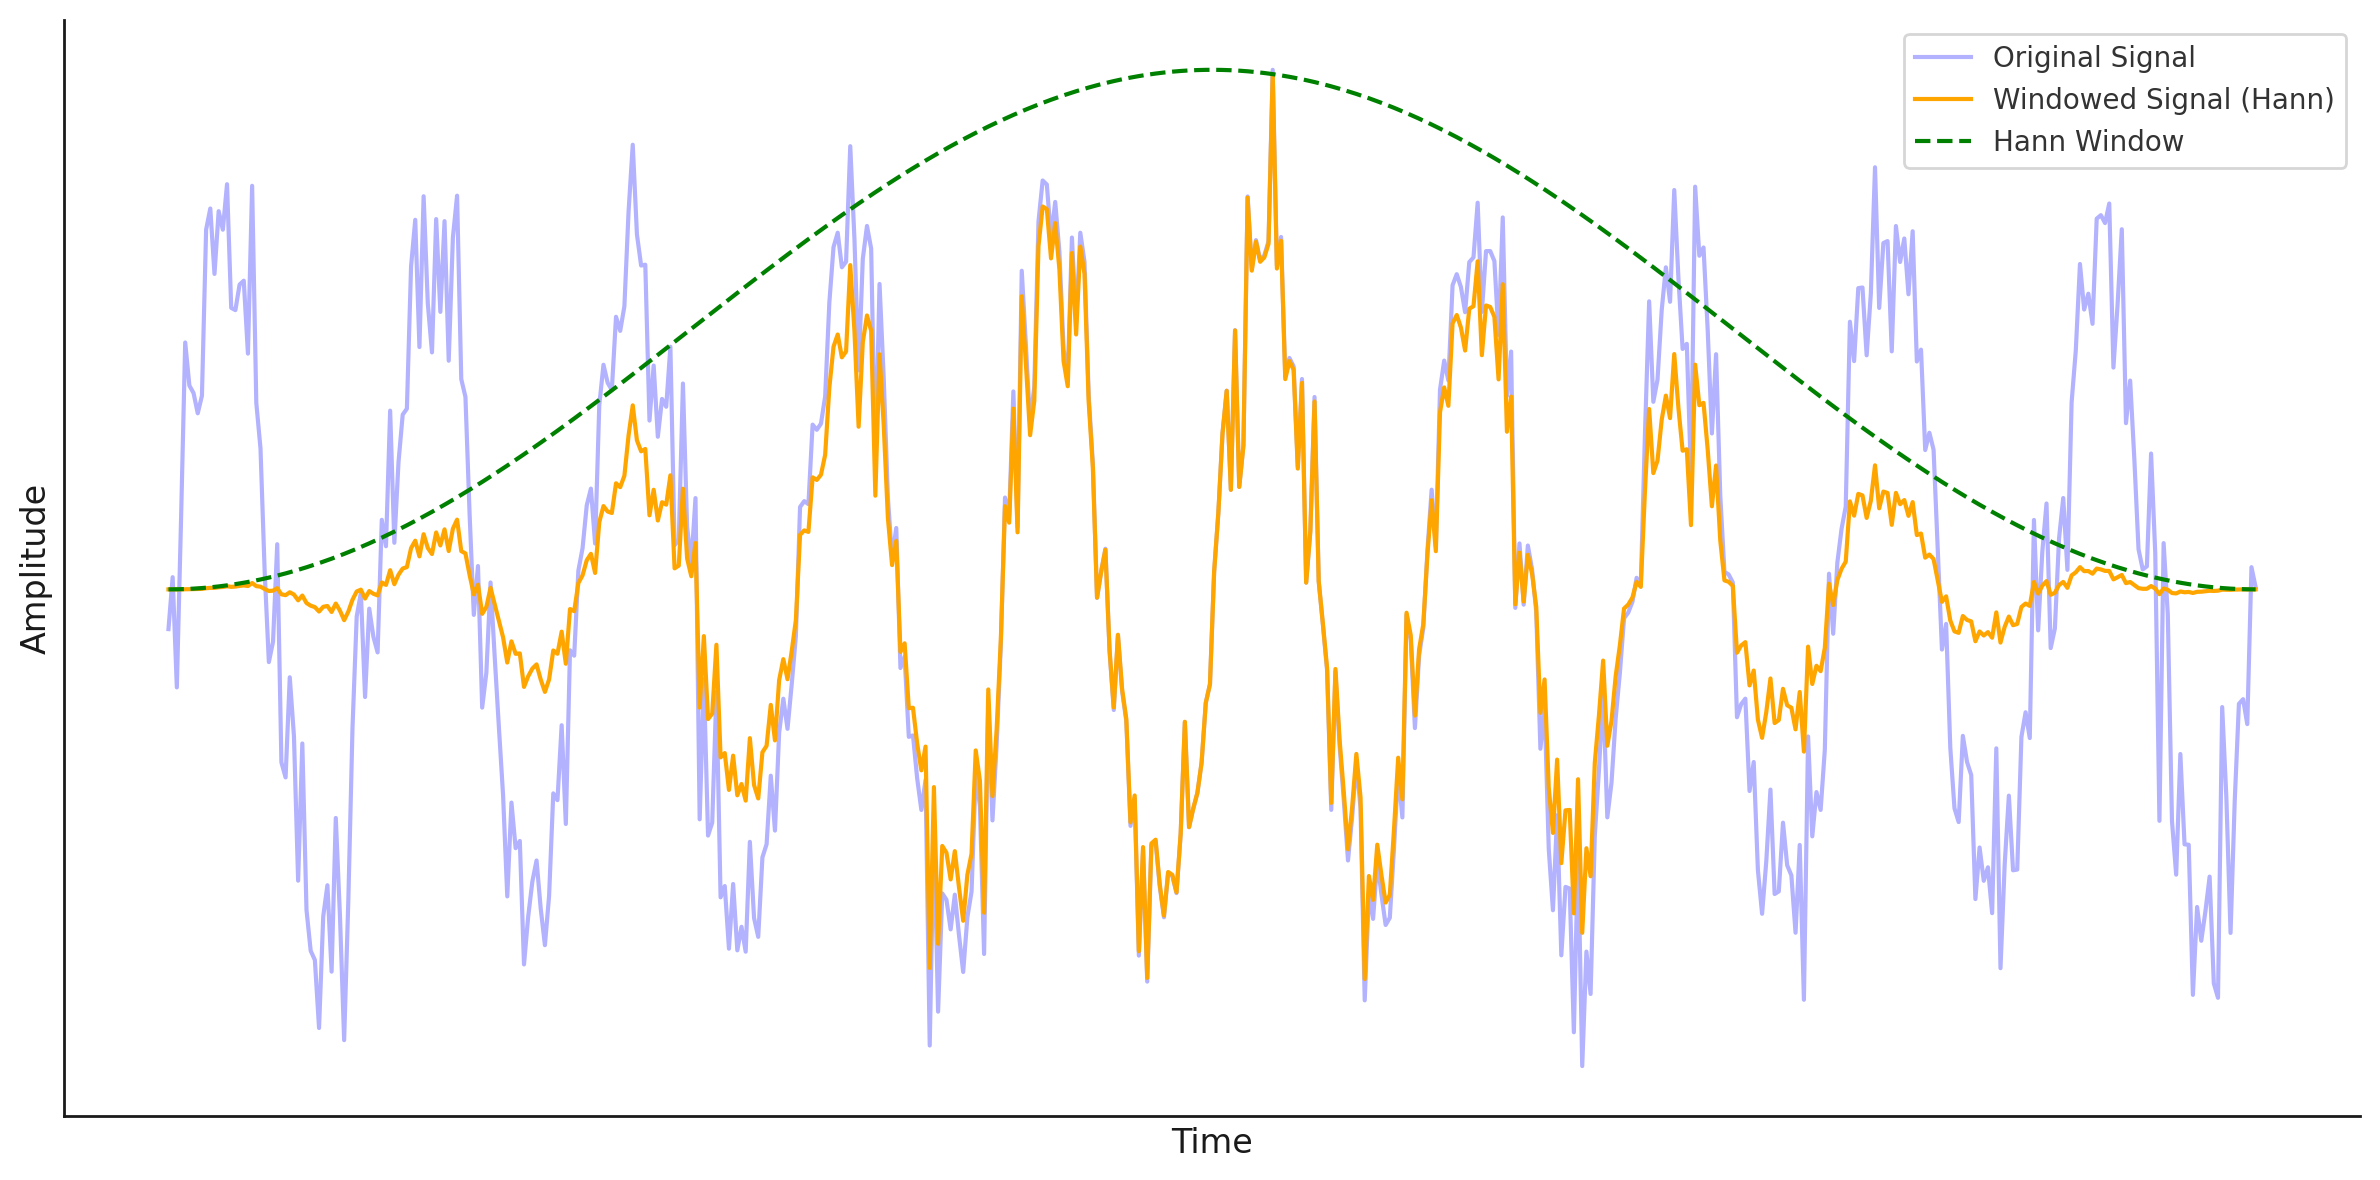
\includegraphics[width=0.8\linewidth]{Chapters/struktura_sustava/generiranje_znacajki/hann.png} 
    \caption{Hannov prozor}
    \label{pic:hann}
\end{figure}

Opisani postupak množenja originalnog signala Hannovim prozorom prikazan je 
matematičkim izrazom \ref{eq:window}.

\begin{equation}
    x_w[n] = x[n] \cdot w[n]
    \label{eq:window}
\end{equation}

gdje je:
\begin{itemize}
    \item \( x_w[n] \) signal nakon primjene Hann prozora,
    \item \( x[n] \) originalni diskretni signal,
    \item \( w[n] \) Hann prozor definiran kao:
    \begin{equation}
        w[n] = 0.54 - 0.46 \cdot \cos\left( \frac{2 \pi n}{N-1} \right)
    \end{equation}
    za \( n = 0, 1, 2, \dots, N-1 \),
    gdje je \( N \) ukupni broj uzoraka u prozoru.
\end{itemize}

Budući da su uzorci tipa \texttt{int16\_t} (16-bitni broj), raspon vrijednosti signala 
prije množenja s funkcijom prozora je [$-2^{15}$, $2^{15} - 1$], tj. [-32768, 32767]. Uz množenje
signala funkcijom prozora, cijelokupni signal skalirat ćemo na raspon [-1, 1] dijeljenjem svakog
uzorka s 32768. Dobiveni signal veličine WINDOW\_SIZE i tipa \texttt{float} (realni broj) je nakon
opisane obrade spreman za spektralnu analizu koja podrazumijeva korištenje diskretne Fourierove
transformacije.

\subsubsection{Diskretna Fourierova transformacija}
\label{sec:fft}

Diskretna Fourierova transformacija (engl. Discrete Fourier Transform ili DFT) matematička je
funkcija koja se koristi za analizu diskretnih signala u frekvencijskoj domeni. 
DFT diskretnog signala \( x[n] \) s \( N \) uzoraka definirana je izrazom \ref{eq:dft}.

\begin{equation}
    X[k] = \sum_{n=0}^{N-1} x[n] e^{-j 2 \pi k n / N}, \quad k = 0, 1, \dots, N-1
    \label{eq:dft}
\end{equation}

gdje je:
\begin{itemize}
    \item \( X[k] \): spektralni koeficijent na \( k \)-toj frekvenciji,
    \item \( x[n] \): signal u vremenskoj domeni,
    \item \( N \): broj uzoraka signala,
    \item \( e^{-j 2 \pi k n / N} \): osnovni eksponencijalni faktor.
\end{itemize}

Međutim, računalno je zahtjevna te se zbog toga koristi puno brži algoritam izračuna
frekvencijskih komponenata koji se zove Brza Fourierova transformacija (engl. Fast Fourier
Transform ili FFT). To je učinkovita računalna implementacija DFT-a koja značajno smanjuje
broj operacija potrebnih za izračun koeficijenata spektra.

Na mikrokontrolerskom sustavu koji se koristi za implementaciju cjelokupnog sustava
dostupne su funkcije koje izračunavaju spektralne koeficijente za dani signal. 
Programski kod \ref{code:fft} prikazuje inicijalizacijski kod potreban za pravilnu 
upotrebu FFT-a te metodu \texttt{void FFT::compute(float* frame, float* spectrogram)} 
razreda FFT koja izračunava koeficijente koji predstavljaju kvadratnu vrijednost
amplitude svake frekvencijske komponente (spektar snage signala) kojih ima 
WINDOW\_SIZE / 2 + 1 (još definirano kao NUMBER\_OF\_SPECTROGRAM\_BINS). 
Funkcija prima pokazivač na prozor (\texttt{float* frame}) te pokazivač na polje
u koje će biti spremljen rezultat FFT-a (\texttt{float* spectrogram}). Izlazna
varijabla je imena \texttt{spectrogram} jer spektralnom analizom signala dobijemo
nešto što se zove spektrogram. Preciznije, spektrogram bi će biti dvodimenzionalno
polje koje sadrži više ovakvih jednodimenzionalnih vektora koje dobijemo nakon
Fourierove transformacije jednog prozora. 

\begin{lstlisting}[language=C++, caption=FFT, label=code:fft]
    // initialization 
    dsps_fft2r_init_fc32(NULL, WINDOW_SIZE);
    void FFT::compute(float* frame, float* spectrogram) {
        for(size_t i = 0; i < WINDOW_SIZE; i++) {
            data[2 * i] = frame[i];  // Real part
            data[2 * i + 1] = 0;     // Imaginary part
        }
        // Perform FFT
        dsps_fft2r_fc32_ae32(data, WINDOW_SIZE);
        // Bit reversal
        dsps_bit_rev_fc32_ansi(data, WINDOW_SIZE);
        // Magnitude (power) of each frequency bin
        for(size_t i = 0; i < NUMBER_OF_SPECTROGRAM_BINS; i++) {
            float real = data[2 * i];
            float imag = data[2 * i + 1];
            spectrogram[i] = sqrt(real * real + imag * imag);
        }
    }
\end{lstlisting}


\subsubsection{Melovo skaliranje}
\label{sec:mel}
Izlaz iz modula koji se bavi Fourierovom transformacijom je frekvencijski spektar signala.
Preciznije svaki element tog vektora je amplituda snage određene frekvencije sadržane u signalu.
Te frekvencije su raspoređene linearno. Međutim, čovjek ne percipira jednako male promjene 
na višim frekvencijama isto kao na nižim. Zbog toga je potrebno na neki način skalirati
razmake između frekvencija kako bi bolje odgovarali ljudskoj percepciji. Za potrebe toga
osmišljena je Melova skala (engl. Mel scale). Preslikavanje na takvu skalu opisano je formulom
\ref{eq:mel}.

\begin{equation}
    m(f) = 2595 \cdot \log_{10}\left(1 + \frac{f}{700}\right)
    \label{eq:mel}
\end{equation}

gdje je:
\begin{itemize}
    \item \(m(f)\) frekvencija u Mel skali,
    \item \(f\) frekvencija u Hertzima.
\end{itemize}

Na slici \ref{pic:mel} prikazano je preslikavanje iz Hz ljestvice u Melovu. Vidljivo je da
jednake promjene frekvencije u Hertzima na višim frekvencijama odgovaraju manjoj promjeni 
na Mel skali nego na nižim frekvencijama (logaritamsko preslikavanje), a to izravno
odgovara ljudskoj percepciji koja je osjetljivija na promjene u nižim dijelovima spektra.

\begin{figure}[htb]
    \centering
    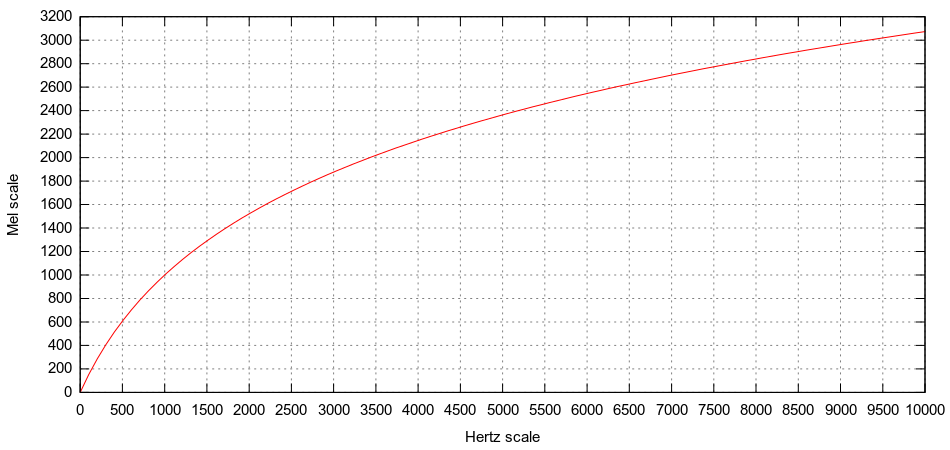
\includegraphics[width=0.8\linewidth]{Chapters/struktura_sustava/generiranje_znacajki/mel.png} 
    \caption{Melova skala \cite{mel}}
    \label{pic:mel}
\end{figure}

Budući da je naš sustav diskretan, postoji prirodni broj frekvencijskih komponenti koje 
dobijemo na izlazu iz Fourierove transformacije (NUMBER\_OF\_SPECTROGRAM\_BINS) koji
izravno ovisi o broju točaka nad kojima se vrši FFT. Sljedeći korak koji je potreban je
napraviti preslikavanje iz Hz ljestvice u Melovu. Prije početka preslikavanja, potrebno
je odrediti rezoluciju preslikavanja, tj. koliko spektralnih komponenti želimo na 
novoj (Melovoj) ljestvici. Taj parametar također je određen u konfiguracijskoj datoteci
\texttt{Configuration.hpp}, a zove se NUMBER\_OF\_MEL\_BINS (u prijevodu broj Melovih
kanti). Samo preslikavanje se odrađuje pomoću trokutaskih filtara prikazanih na slici 
\ref{pic:melfilter}.

\begin{figure}[htb]
    \centering
    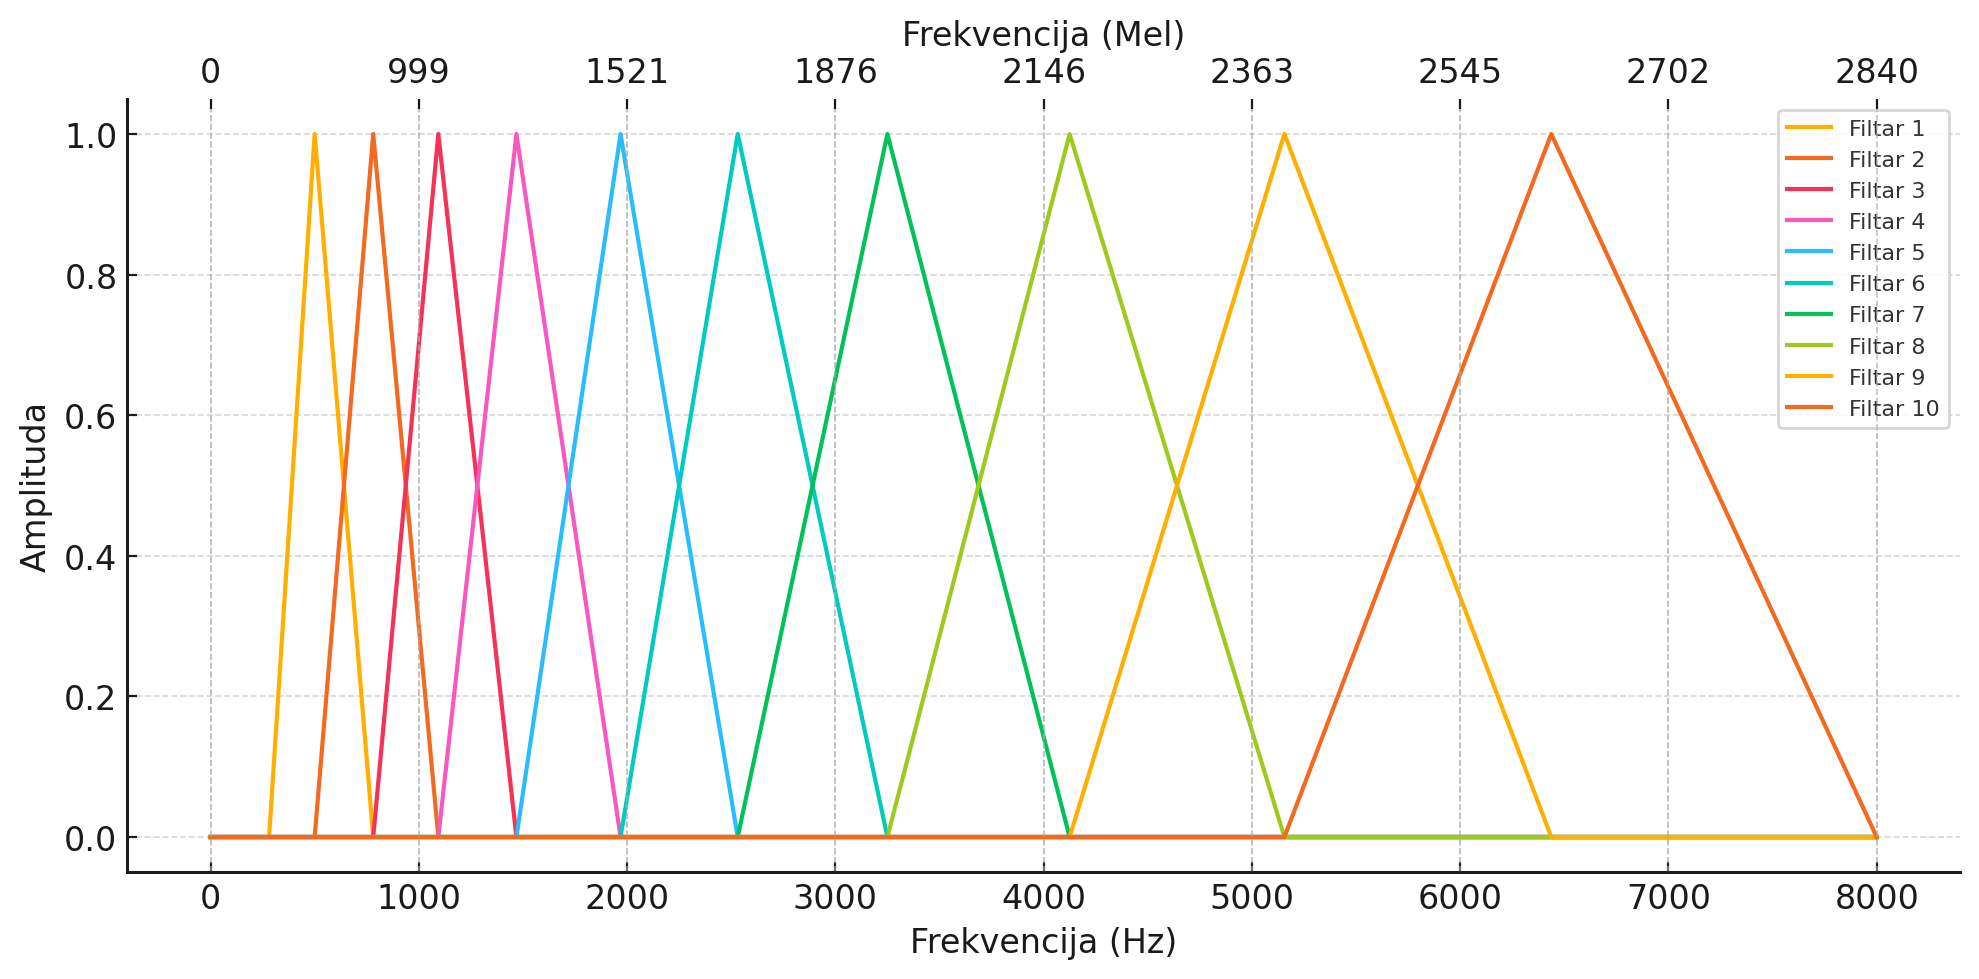
\includegraphics[width=0.8\linewidth]{Chapters/struktura_sustava/generiranje_znacajki/melfiltar.png} 
    \caption{Filtri za Melovu skalu}
    \label{pic:melfilter}
\end{figure}

Za potrebe sustava za prepoznavanje glasa, određuju se donja i gornja granica preslikavanja 
(LOWER\_BAND\_LIMIT i UPPER\_BAND\_LIMIT) koje su tijekom cijelog razvoja sustava "zacementirane"
na 80 Hz i 7600 Hz (takve granice su se pokazale prikladne za ovu svrhu). Od donje do gornje
granice, linearno (na Mel skali) se raspoređuju sredine filtara čija je širina na svaku stranu 
točno do sredine susjednog filtra. Izvan tog intervala vrijednost filtra je nula, dok je u središtu
pojedinog filtra vrijednost istoga točno jedan. Nadalje, vrijednosti svake Melove frekvencijeske
komponente doprinosi vrijednost frekvencijske komponente s Hz ljestvice onoliko koliko iznosi
njena vrijednost pomnožena s vrijednosti filtra na tom mjestu. Za svaki filtar (koji odgovara
jednoj Mel frekvencijskoj komponenti) potrebno je provjeriti koliko svaka frekvencijska komponenta 
s Hz ljestvice doprinosi toj Mel komponenti, tj. koliko energije iz početnog signala
odgovara toj komponenti na Melovoj ljestvici. Programski kod koji se bavi opisanim prikazan je u 
\ref{code:mel}. Na kraju cjelokupnog procesa, potrebno je svaku vrijednost Melovih frekvencijskih
komponenti logaritmirati jer je to potrebno za sljedeći korak, a to je generiranje MFC koeficijenata.

\begin{lstlisting}[language=C++, caption=FFT, label=code:mel]
void MelSpectrogram::generate(float *spectrogram, float *melSpectrogram){
    for (int melBin = 0; melBin < NUMBER_OF_MEL_BINS; melBin++) {
        melSpectrogram[melBin] = 0.0;
        for (int fftBin = 0; fftBin < NUMBER_OF_SPECTROGRAM_BINS; fftBin++){
            float freq = fftBin * hzPerBin;
            float weight = 0.0;

            if (freq >= melPoints[melBin] && freq < melPoints[melBin + 1]){
                weight = (freq - melPoints[melBin]) / (melPoints[melBin + 1] - melPoints[melBin]);
            } else if (freq >= melPoints[melBin + 1] && freq < melPoints[melBin + 2]){
                weight = (melPoints[melBin + 2] - freq) / (melPoints[melBin + 2] - melPoints[melBin + 1]);
            }

            melSpectrogram[melBin] += spectrogram[fftBin] * weight;
        }
        // Apply log scaling with a safeguard against log(0)
        melSpectrogram[melBin] = logf(fmaxf(melSpectrogram[melBin], 1e-6));
    }
}
\end{lstlisting}

\subsubsection{Diskretna kosinusna transformacija}

Posljednji korak u procesu generiranja Mel kepstralnih koeficijenata (MFCC) je primjena diskretne
kosinusne transformacije (engl. Discrete Cosine Transform ili DCT) na vektor Melovih spektralnih
koeficijenata. Ona pretvara signal iz vremenske ili frekvencijske domene u 
domenu kosinusnih komponenti. Rezultat DCT-a je niz koeficijenata koji predstavljaju energiju 
signala u različitim frekvencijskim opsezima. 
Postoje različiti tipovi DCT-a, ali za MFCC se najčešćee koristi DCT-II koja je prikazana
formulom \ref{eq:dct}.

\begin{equation}
    \label{eq:dct}
    C(k) = \sqrt{\frac{2}{N}} \sum_{n=0}^{N-1} X(n) \cdot \cos\left[ \frac{\pi}{N} \left(n + \frac{1}{2}\right) k \right], \quad k = 0, 1, \dots, N-1
\end{equation}
Gdje su:
\begin{itemize}
\item $C(k)$: koeficijenti DCT-a (u našem slučaju MFCC)
\item $X(n)$: ulazni Mel-frekvencijski spektar,
\item $N$: broj uzoraka u ulaznom spektru,
\item $k$: indeks koeficijenta (MFCC-a).
\end{itemize}

U kontekstu generiranja MFCC-a, ulaz u DCT dolazi iz Mel-frekvencijskog spektra, koji je već 
logaritamski skaliran kako bi pratio ljudsku percepciju glasnoće. Primjenom DCT-a na ovaj spektar 
postiže se:

\begin{enumerate}
\item \textbf{Dekorelacija podataka}: Komponente Mel-frekvencijskog spektra obično su jako 
korelirane. DCT uklanja ovu korelaciju, što omogućuje jednostavniju analizu i smanjuje
redundantnost.

\item \textbf{Redukcija dimenzionalnosti}: DCT generira niz koeficijenata, ali samo prvih
nekoliko (obično 12-13) sadrže značajne informacije potrebne za prepoznavanja govora ili zvukova. 
Ostatak koeficijenata se odbacuje jer sadrže manje bitne informacije ili šum.

\item \textbf{Efikasnija obrada}: Kompresijom podataka DCT smanjuje zahtjeve za memorijom i 
procesorskom snagom (sva informacija prozora podataka sadržana je u ovih 12 ili 13 koeficijenata).
\end{enumerate}

Implementacija  diskretne kosinusne transformacije prikazana je u odječku koda \ref{code:dct}.
U konstruktoru razreda DCT inicijaliziraju se koeficijenti potrebni za izračun pojedinog MFCC-a,
dok metoda compute računa MFCC-e za konkretni ulzni Mel-frekvencijski spektar. Na taj način
razdvojen je izračun na dva dijela: konstanti dio koji ne ovisi o ulaznom spektru (računa
se pri konstrukciji objekta zaduženog za DCT) i dio koji
ovisi o ulaznom spektru te ga je zbog toga potrebno računati u svakoj iteraciji.\newline{}


\begin{lstlisting}[language=C++, caption=FFT, label=code:dct]
DCT::DCT()
{
    const float pi = 3.14159265358979323846f;
    for (int i = 0; i < NUMBER_OF_MFCCS; ++i) {
        for (int j = 0; j < NUMBER_OF_MEL_BINS; ++j) {
            coefficients[i * NUMBER_OF_MEL_BINS + j] = cos(pi * i * (j + 0.5f) / NUMBER_OF_MEL_BINS);
        }
    }
}

void DCT::compute(const float *input, float *output) {
    for (int i = 0; i < NUMBER_OF_MFCCS; i++) {
        output[i] = 0.0;
        for (int j = 0; j < NUMBER_OF_MEL_BINS; j++) {
            output[i] += input[j] * coefficients[i * NUMBER_OF_MEL_BINS + j];
        }
        output[i] *= sqrt(2.0 / NUMBER_OF_MEL_BINS);
    }
}
\end{lstlisting}

Konačni rezultat cijelog procesa generiranja značajki je NUMBER\_OF\_MFCCS Mel kepstralnih
koeficijenata. Zašto se tako zovu? Melovi su jer su bazirani na Melovoj frekvencijskoj
skali koja je ubjašnjena u \ref{sec:mel}. Međutim zašto su kepstralni možda nije intuitivno.
Dolazi od toga što smo tokom njihovih generiranja morali posegnuti za dvama transformacijama.
Prva je bila FFT. Ona je signal iz vremenske domene prebacila u frekvencijsku (spektar
signala). Druga transformacija je bila upravo DCT. Ona je još jednom računala spektar, međutim
ovog putaje je to bio spektar spektra. Zbog toga su koeficijenti it ove domene dobili ime
kepstralni (keps je anagram od spek). Ovo sve se može povezati s modelom govora opisanog
u \ref{sec:speech}. Spektar spektra nam omogućuje razdvajanje energija u pojedinim 
frekvencijskim spektrima te jako dobro razdvaja odziv vokalnog trakta od kvazi-periodičnog
impulsa. Također, informaciju zvučnog prozora duljine WINDOW\_SIZE komprimirali smo
u svega NUMBER\_OF\_MFCCS Mel kepstralnih koeficijenata. Te veličine mogu varirati, a
karakteristični iznosi u sustavima ovakvog tipa su redom 512 te 13. To je svega oko 2.5\% 
broja početnih značajki (5\% ako se promatra memorijsko zauzeće jer float tip varijable
zauzima 4 bajta, dok int16\_t zauzima 2 bajta). Blok dijagram cjelokupnog procesa prikazan
je na slici \ref{pic:generation}.

\begin{figure}[htb]
    \centering
    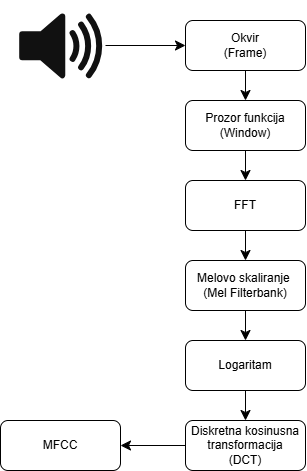
\includegraphics[width=0.4\linewidth]{Chapters/struktura_sustava/generiranje_znacajki/generation.png} 
    \caption{Proces generiranja MFCC-a \cite{flowchart}}
    \label{pic:generation}
\end{figure}

\subsection{Konstrukcija matrice značajki}
\label{sec:featureImage}
U poglavlju \ref{MFCCconstruction} opisana je konstrukcija MFC koeficijenata iz jednog
okvira zvučnog zapisa tipične duljine od oko 20 do 30 ms \cite{wardentinyml}. 
Na način koji je opisan u
\ref{sec:win} u sljedećoj iteraciji dohvatit će se određeni broj novih uzoraka koji će
sudjelovati u stvaranju novog okvira nad kojim je 
potrebno generirati nove Mel kepstralne koeficijente koji odgovaraju tom prozoru na način
identičan opisanom. Proces dohvaćanja novih uzoraka te generiranje novih MFCC-a kontinuirano
se ponavlja kroz cijeli vijek rada uređaja. Rezultat generiranja značajki je 
jednodimenzionalni vektor koji sadrži NUMBER\_OF\_MFCCS koeficijenata. Tako generirane značajke
je potrebno predati podsustavu koji je zadužen za aktivaciju neuronske mreže. Konkretno,
sustav za prepoznavanje koristi konvolucijsku neuronsku mrežu čija je stuktura te 
područje primjene podrobnije opisano u \ref{sec:cnn}. One dobro funkcioniraju u klasifikaciji
višedimenzionalnih matrica. Ideja je primijeniti takvu strukturu na značajke koje su prethodno
generirane. Uzastopni vektori MFC koeficijenata slagani su u dvodimenzionalnu matricu koja
onda može biti predana neuronskoj mreži. Možemo reći da je takvim slaganjem dobivena slika
zvučnog zapisa proizvoljne dujine! Što će odrediti koliko će prozora podataka biti u jednom 
trenutku predano na klasifikaciju? Pa upravo duljina podataka nad kojima je mreža i trenirana!
Detaljniji opis skupa podataka za treniranje mreže nalazi se u \ref{sec:dataset}, najbitnije
za reći ovje je da se radi o skupu zvučnih zapisa u trajanju od jedne sekunde. Zbog toga
je potrebno napraviti matricu od onoliko prozora koliko je potrebno da pokriju
vrijeme od 1 sekunde. Broj takvih prozora NUMBER\_OF\_TIME\_SLICES će ovisiti
o veličini prozora WINDOW\_SIZE,
broju novih uzoraka u svakoj iteraciji STEP\_SIZE te frekvenciji otipkavanja
SAMPLE\_RATE. Funkcija \ref{eq:timeslices} opisuje opisanu ovisnost.

\begin{equation}
    \label{eq:timeslices}
    \text{NUMBER\_OF\_TIME\_SLICES} = \left\lfloor \frac{\text{SAMPLE\_RATE} - \text{WINDOW\_SIZE}}{\text{STEP\_SIZE}} \right\rfloor + 1
\end{equation}

Budući da se konstantno akviziraju novi podaci te generiraju njihove značajke, a veličina
dvodimenzionalne matrice koja se predaje neuronskoj mreži ostaje stalna, potrebno je 
dolaskom značajki novog vremenskog prozora, odbaciti najstariji, ostale pomaknuti prema početku
te na kraj matrice dodati najnovije značajke. Algoritam je vrlo sličan onom koji novoakvizirane
uzorke dodaje na kraj vremenskog prozora prije generiranja značajki, a prikazan je u odsječku
programskog koda \ref{code:featureImage}. U polje \texttt{featureSlice} se spremaju novonastale
značajke, a polje \texttt{featureImage} sadrži trenutno dvodimenzionalno polje značajki (ovdje je
je definirano kao jedodimenzionalno, međutim memorijski otisak je identičan i, ono najbitnije,
takva struktura odgovara ulazu neuronske mreže). Veličina tog polja NUMBER\_OF\_FEATURES je samo
umnožak broja značajki pojedinog prozora NUMBER\_OF\_MFCCS i broja prozora potrebnog za 
izgradnju matrice NUMBER\_OF\_TIME\_SLICES.

\begin{lstlisting}[language=C++, caption=Generiranje matrice značajki, label=code:featureImage]
    float featureSlice[NUMBER_OF_MFCCS] = {0};
    float featureImage[NUMBER_OF_FEATURES] = {0};

    memcpy(featureImage, featureImage + NUMBER_OF_MFCCS, sizeof(float) * (NUMBER_OF_FEATURES - NUMBER_OF_MFCCS));
    memcpy(featureImage + NUMBER_OF_FEATURES - NUMBER_OF_MFCCS, featureSlice, sizeof(float) * NUMBER_OF_MFCCS);
\end{lstlisting}

Algoritam osvježavanja postojeće matrice značajki prikazan je slikom \ref{pic:featureImage}. 
Pokazna matrica se sastoji od sedam vremenskih odsječaka i šest MFC koeficijenata. Crveni 
vremenski prozor značajki se dodaje je na kraj matrice, dok se istovremeno ostali pomiču prema
naprijed te istiskuju najstariji prozor koji je u ovom slučaju obojan plavom bojom.

\begin{figure}[htb]
    \centering
    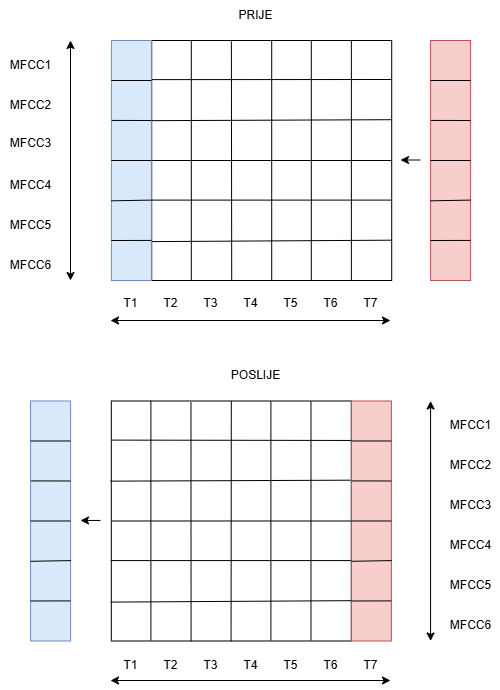
\includegraphics[width=0.5\linewidth]{Chapters/struktura_sustava/generiranje_znacajki/featureImage.png} 
    \caption{Matrica značajki \cite{flowchart}}
    \label{pic:featureImage}
\end{figure}
\section{Aktivacija neuronske mreže}
\label{sec:activation}

Aktivacija neuronske mreže (engl. invoking) proces je u kojem se ulaznom sloju neuronske mreže 
(engl. input layer) predaje matrica značajki. Biblioteka koja je korištena za implementaciju
neuronske mreže na mikrokontroleru je TensorFlow Lite \ref{tflm}. Omogućuje vrlo jednostavno
korištenje treniranog modela (treniranog na računalu kako je opisano u ... te konvertiranog
u polje koje se može koristiti na mikrokontroleru kako je opisano u ...). Trenirani model
je polje 8-bitnih vrijednosti koje predstavljaju pojedine parametre mreže dobivene upravo 
treniranjem modela. Razred koji omotava korištenje biblioteke i modela prikazan je 
u isječku koda \ref{code:NeuralNetwork}. 

\begin{lstlisting}[language=C++, caption=Razred neuronske mreže, label=code:NeuralNetwork]
class NeuralNetwork
{
    private:
        const tflite::Model* model = nullptr;
        tflite::MicroInterpreter* interpreter = nullptr;
        TfLiteTensor* model_input = nullptr;
        uint8_t tensor_arena[TENSOR_ARENA_SIZE];
        tflite::MicroMutableOpResolver<N> resolver;
        float* model_input_buffer = nullptr;
    public:
        NeuralNetwork();
        void giveFeaturesToModel(float* features, size_t numberOfFeatures);
        bool invoke(void);
        int numberOfClasses;
        float* outputData;  
};   
\end{lstlisting}

\texttt{const tflite::Model* model} predstavlja 
pokazivač na polje parametara modela, dok \texttt{tflite::MicroMutableOpResolver<N> resolver}
predstavlja arhitekturu neuronske mreže. Toj strukturi je potrebno dodati sve vrste slojeva 
i funkcija koje se koriste unutar arhitekture mreže koja je trenirana. Primjer dodavanja 
nekih vrsta slojeva prikazan je u isječku koda \ref{code:resolver}. Nije bitan redoslijed 
dodavanja, samo je potrebno dodati sve što ta mreža sadrži.

\begin{lstlisting}[language=C++, caption=Gradnja arhitekture mreže, label=code:resolver]
resolver.AddConv2D()            // konvolucijski sloj
resolver.AddFullyConnected()    // potpuno povezani sloj
resolver.AddSoftmax()           // softmax funkcija
resolver.AddMaxPool2D()         // sloj za poduzorkovanje
\end{lstlisting}

Nakon što je mreža alocirana na pravilan način (struktura polja u kojem se nalaze parametri
mreže odgovara strukturi mreže na mikrokontroleru) moguće joj je predati matricu značajki
te ju aktivirati. Nakon aktivacije, mreža "provlači" vrijednosti kroz svoju strukturu te na
izlazu daje vjerojatnosti da određeni ulaz (matrica značajki) predstavlja naučenu naredbu. 
Kako je objašnjeno u \ref{sec:data}, broj kategorija za koje trenirana mreža daje na izlazu
vjerojatnosti je za dva veći od broja naredbi koje mreža može prepoznati. Dodatne kategorije
su "pozadina" (engl. background) i "nepoznato" (engl. unknown). 

Aktivacija neuronske mreže i dobivanje vrijednosti na njenom izlazu, koje predstavljaju
vjerojatnosti da ulazna matrica značajki pripada određenoj kategoriji, samo je jedna iteracija 
u radu sustava čija je struktura prikazana slikom \ref{pic:struktura_sustava}. Svakom novom 
iteracijom rada sustava, akviziraju se novi zvučni uzorci, matrica značajki se osvježava, 
tj. noviji MFC koeficijenti dolaze u matricu. Novi podaci u matrici predstavljaju značajke 
signala pomaknutog za dohvaćeni broj uzoraka (tipično 20-30 milisekundi) te je potrebno provjeriti
kojoj kategoriji pripada taj vremenski prozor. Budući da je od aktivacije mreže do izlaska 
rezultata u krajnjem sloju mreže potrebno određeno vrijeme, nije moguće aktivirati mrežu 
na svaki novi vremenski prozor podataka jer će biti zagušeno akviziranje novih podataka
te cjelokupni sustav neće dobro raditi u stvarnom vremenu. Međutim, dobra vijest je da
nije potrebno aktivirati mrežu na svaki novi vremenski korak jer je on svojom duljinom
puno manji od duljine uzorka kojeg predstavlja cijela matrica. Drugim riječima, uzastopne
verzije ulazne matrice podataka će biti vrlo slične i možemo pričekati nekoliko novih
iteracija prije nego li aktiviramo neuronsku mrežu (akviziranje signala i generiranje značajki
tipično traje puno kraće od aktivacije). S druge strane, mreža se mora aktivirati dovoljno
često jer u suprotnom postoji mogućnost propusta određeni naredbi. Parametar koji brine o tome 
koliko često se mreža aktivira zove se NUMBER\_OF\_NEW\_SLICES\_BEFORE\_INVOKING i određen
je eksperimentalno zbog toga što drugačije strukture mreže imaju drugačije vrijeme odziva.
Potrebno je maksimizirati broj aktiviranja mreže u određenom vremenu bez da se gube
uzorci ulaznog signala.

\begin{figure}[htb]
    \centering
    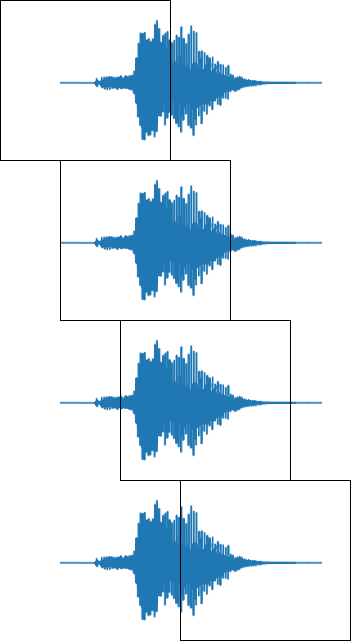
\includegraphics[width=0.4\linewidth]{Chapters/struktura_sustava/aktivacija_nn/timeline.png}
    \caption{Uzastopni vremenski okviri (prozori) \cite{flowchart}}
    \label{pic:timeline}
\end{figure}

Na slici \ref{pic:timeline} prikazani su uzastopni vremenski prozori nad ulaznim zvučnim signalom.
Na signalu je vidljiv vremenski odsječak u kojem je izgovorena naredba, a prije i poslije
izgovorene naredbe je tišina. U drugom i trećem prozoru očekuje se velika vjerojatnost da 
je prepoznata izgovorena naredba, dok se u prvom i četvrtom prozoru ne očekuje prepoznavanje
određene naredbe (u tim prozorima veću vjerojatnost imaju kategorije "nepoznato" ili "pozadina").
Upravo zbog prikazanog je potrebno što češće aktivirati mrežu i ne propustiti prepoznavanje naredbe. 
U slučaju da smo aktivirali mrežu rjeđe, ne bismo prepoznali naredbu (npr. prvi pa četvrti
prozor). 

No, takav pristup otvara mjesto drugom problemu. Ne želimo niti višestruko prepoznavanje
jednom izgovorene naredbe. Tu na scenu stupa podsustav za prepoznavanje i okidanje naredbi.
\section{Prepoznavanje naredbi i aktivacija zadatka}
\label{sec:prepoy}

Ako se mreža aktivira dovoljno često, za očekivati je da će najvjerojatniji izlaz iz 
neuronske mreže u slučaju izgovorene naredbe biti upravo kategorija koja predstavlja tu naredbu. 
Štoviše, naredba bi trebala biti prepoznata u više uzastopnih iteracija aktiviranja mreže.
Međutim, ponašanje sustava u tom slučaju neće biti onakvo kakvo bi trebalo biti, a to je da se
određeni posao (zadatak) aktivira isključivo jednom za jednom izgovorenu naredbu. 
Dodatno treba pripaziti na slučajno aktiviranje nekog posla jer zbog
nesavršenosti mreže se može dogoditi da vjerojatnosni izlaz ukazuje na prepoznavanje neke
naredbe, iako se ona u stvarnosti nije izgovorila. Međutim, u takvim situacijama se očekuje možda jedna ili dvije takve situacije zaredom,
ali ne i više njih. Zbog svega navedenog, potrebno je na neki način obraditi tok vjerojatnosnih
izlaza iz neuronske mreže. Kao najbolji način za pokrivanje svih problema pokazalo se 
uprosječivanje vjerojatnosti pojedinih kategorija. 

Na slici \ref{pic:uml} prikazan je UML dijagram implementiranog podsustava. Upravljački dio posla
obavlja se unutar razreda \texttt{CommandRecognizer} koji je zadužen za aktiviranje obavljanja 
konkretnog posla koji je povezan s govornom naredbom. 
Sadrži listu pokazivača na objekte čiji razredi implementiraju 
sučelje \texttt{Command}. \texttt{Command} predstavlja sučelje (apstraktni razred) što znači da
nije moguće konstruirati objekt tog razreda, nego da je potrebno naslijediti razredom koji 
implementira apstraktnu metodu \texttt{virtual void execute(float probability)}. Ta 
metoda je zadužena za obavljanje konkretnog zadatka. Ovakav strukturni
obrazac daje mogućnost vrlo lakog implementiranja novih vrsta zadataka (sve što je potrebno je 
napraviti novi razred koji implementira sučelje \texttt{Command}, tj. nadjačava
spomenutu metodu). Trenutačno su implementirane
dvije vrste naredbi (zadataka): \texttt{BlankCommand} koja ne radi ništa (koristi se za kategorije
\textit{"pozadina"} i \textit{"nepoznato"}) i \texttt{PrintCommand} koja ispisuje ime naredbe i prosječnu 
vjerojatnost pojavljivanja naredbe.

\begin{figure}[htb]
    \centering
    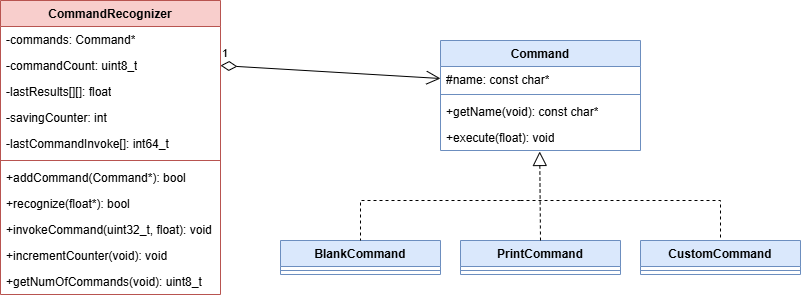
\includegraphics[width=0.9\linewidth]{Chapters/struktura_sustava/prepoznavanje_naredbi/commands.png} 
    \caption{Podsustav za prepoznavanje naredbi i aktivaciju zadataka\cite{flowchart}}
    \label{pic:uml}
\end{figure}

Prilikom konstrukcije objekta razreda koji implementira sučelje \texttt{Command} potrebno je postaviti
parametre za prepoznavanje naredbe koji se utvrđuju eksperimentalno. Parametrom \texttt{historySize}
bira se broj uzastopnih vrijednosti vjerojatnosti pojave naredbe nad kojima se računa prosjek,
a parametar \texttt{threshold} postavlja prag koji prosječna vrijednost mora prijeći kako bi se naredba
aktivirala. Ovim se postiže odvojeno kalibriranje parametara za svaku naredbu koje je potrebno
zbog podataka nad kojima se mreža uči. Zbog nejednakosti kvalitete podataka može se dogoditi da se određene
naredbe prepoznaju lakše ili teže od drugih.
Uz to, objekt razreda \texttt{CommandRecognizer} brine o tome da se naredba aktivira
samo ako je prošlo određeno vrijeme nakon zadnje aktivacije. To se postiže parametrom 
\texttt{COOL\_DOWN\_PERIOD\_MS} koji je definiran u datoteci \texttt{Configuration.hpp} \ref{add:config}.
Jednom konstruirani objekt naredbe potrebno je dodati 
u objekt klase \texttt{CommandRecognizer} metodom \texttt{bool addCommand(Command* command)} 
kako bi znao za postojanje te naredbe (broj izlaza iz neuronske mreže mora odgovarati 
broju dodanih naredbi ovim putem). Svaka konkretna implementacija metode 
\texttt{virtual void execute(float probability)} ne smije trajati predugo jer će unijeti 
kašnjenje u sustav. Ideja je da takva naredba samo pokrene duži posao za koji će onda
biti zadužen neki drugi podsustav.

Ovime je opisana cjelokupna petlja mikrokontrolerskog sustava
koja se neprestano iznova izvršava (slika \ref{pic:struktura_sustava}).
Jedini element u ovom opisu koji nije detaljno opisan je sama neuronska mreža koja
je u biti okosnica cijelog sustava za prepoznavanje glasovnih naredbi. 
U sljedećem poglavlju će stoga biti detaljno opisana sama neuronska mreža na kojoj se temelji sustav.

